\chapter{Implementation}

\section{Level Set Algorithm}\label{levelsetalgorithm}

\subsection{Upwinding}
Equation \eqref{eq:levelsetequation}, the level set equation, needs to be discretized for both sequential and parallel computation. This is done using the \textit{up-wind} differencing scheme. The following explanation of \textit{upwinding} is from \cite{osher2003lsm}.

A first order accurate method for time discretization of equation \eqref{eq:levelsetequation}, is given by the forward Euler method, from \cite{osher2003lsm}:

\begin{equation}
\frac{\phi^{t+\Delta t}-\phi^t}{\Delta t} +F^{t}\cdot{\nabla{\phi^{t}}} = 0
\label{eq:euler1}
\end{equation}

where $\phi^{t}$ represents the current values of $\phi$ at time $t$, $F^{t}$ represents the velocity field at time $t$, and  $\nabla{\phi^{t}}$ represents the values of the gradient of $\phi$ at time $t$. When computing the gradient, a great deal of care must be taken with regards to the spatial derivatives of $\phi$. This is best exemplified by considering the expanded form of equation \eqref{eq:euler1}.

\begin{equation}
\frac{\phi^{t+\Delta t}-\phi^t}{\Delta t} +u^{t}\phi_x^t+v^{t}\phi_y^t+w^{t}\phi_z^t = 0
\label{eq:euler2}
\end{equation}

For simplicity, consider the one dimensional form of equation \eqref{eq:euler2} at a specific grid point $x_i$ 

\begin{equation}
\frac{\phi^{t+\Delta t}-\phi^t}{\Delta t} +u_i^{t}(\phi_x)_i^t = 0
\label{eq:euler3}
\end{equation}

where $(\phi_x)_i$ is the spatial derivative of $\phi$ at $x_i$. The method of characteristics indicates whether to use a forward difference or backwards difference for $\phi$ based on the sign of $u_i$ at the point $x_i$. If $u_i > 0$, the values of $\phi$ are moving from left to right, and therefore backwards difference methods ($D_x^-$) should be used. Conversely, if $u_i<0$, forward difference methods ($D_x^+$) should be used to approximate $\phi_x$. It is this process of choosing which approximation for the spatial derivative of $\phi$ to use based on the sign of $u_i$ that is known as \textit{upwinding}. 

Extending this to three dimensions, from \cite{Lefohn04astreaming}, results in the derivatives below required for the level set equation update. 

\begin{eqnarray}
	D_x &=& (u_{i+1,j,k}-u_{i-1,j,k})/2 \nonumber\\
	D_y &=& (u_{i,j+1,k}-u_{i,j-1,k})/2 \nonumber\\
	D_z &=& (u_{i,j,k+1}-u_{i,j,k-1})/2 \nonumber\\
	D_x^+ &=& u_{i+1,j,k}-u_{i,j,k} \nonumber\\
	D_y^+ &=& u_{i,j+1,k}-u_{i,j,k} \nonumber\\
	D_z^+ &=& u_{i,j,k+1}-u_{i,j,k} \nonumber\\
	D_x^- &=& u_{i,j,k}-u_{i-1,j,k} \nonumber\\
	D_y^- &=& u_{i,j,k}-u_{i,j-1,k} \nonumber\\
	D_z^- &=& u_{i,j,k}-u_{i,j,k-1} \nonumber\\
\end{eqnarray}

$\nabla\phi$ is approximated using the upwind scheme.

\begin{eqnarray}
\nabla\phi_{\max} &=& \left[
  \begin{array}{ c }
     \sqrt{\max(D_x^+, 0)^2 + \max(-D_x^+,0)^2}  \\[2em]
     \sqrt{\max(D_y^+, 0)^2 + \max(-D_y^+,0)^2}  \\[2em]
     \sqrt{\max(D_z^+, 0)^2 + \max(-D_z^+,0)^2}  
  \end{array} \right] \\[2em]
\nabla\phi_{\min} &=& \left[
  \begin{array}{ c }
     \sqrt{\min(D_x^+, 0)^2 + \min(-D_x^+,0)^2}  \\[2em]
     \sqrt{\min(D_y^+, 0)^2 + \min(-D_y^+,0)^2}  \\[2em]
     \sqrt{\min(D_z^+, 0)^2 + \min(-D_z^+,0)^2} 
  \end{array} \right] 
\end{eqnarray}

Finally, depending on whether $F_{i,j,k} > 0$ or $F_{i,j,k} < 0$, $\nabla\phi$ is 

\begin{equation}
\nabla\phi = \left\{ 
\begin{array}{l l}
  ||\nabla\phi_{\max}||_2 & \quad \mbox{if $F_{i,j,k} > 0$}\\
  ||\nabla\phi_{\min}||_2 & \quad \mbox{if $F_{i,j,k} < 0$}\\ \end{array} \right.
\label{eq:finalchoice}
\end{equation}

\begin{equation}
\phi(t+\Delta t) =\phi(t) + \Delta t F|\nabla\phi|
\label{eq:phi}
\end{equation}

The speed term $F$, as discussed before, is based on the pixel intensity values and curvature values. 

\subsection{Curvature}
Curvature is computed based on the values of the current level set using the derivatives below. In two dimensions only the first two derivatives are required, alongside the derivatives defined previously. In three dimensions, all the derivatives below are required.

\begin{eqnarray}
	D_x^{+y} &=& (u_{i+1,j+1,k}-u_{i-1,j+1,k})/2 \nonumber\\
	D_x^{-y} &=& (u_{i+1,j-1,k}-u_{i-1,j-1,k})/2 \nonumber\\
	D_x^{+z} &=& (u_{i+1,j,k+1}-u_{i-1,j,k+1})/2 \nonumber\\
	D_x^{-z} &=& (u_{i+1,j,k-1}-u_{i-1,j,k-1})/2 \nonumber\\
	D_y^{+x} &=& (u_{i+1,j+1,k}-u_{i+1,j-1,k})/2 \nonumber\\
	D_y^{-x} &=& (u_{i-1,j+1,k}-u_{i-1,j-1,k})/2 \nonumber\\
	D_y^{+z} &=& (u_{i,j+1,k+1}-u_{i,j-1,k+1})/2 \nonumber\\
	D_y^{-z} &=& (u_{i,j+1,k-1}-u_{i,j-1,k-1})/2 \nonumber\\
	D_z^{+x} &=& (u_{i+1,j,k+1}-u_{i+1,j,k-1})/2 \nonumber\\
	D_z^{-x} &=& (u_{i-1,j,k+1}-u_{i-1,j,k-1})/2 \nonumber\\
	D_z^{+y} &=& (u_{i,j+1,k+1}-u_{i,j+1,k-1})/2 \nonumber\\
	D_z^{-y} &=& (u_{i,j-1,k+1}-u_{i,j-1,k-1})/2 \nonumber\\
\end{eqnarray}

Using the \textit{difference of normals} method from \cite{Lefohn04astreaming}, curvature is computed using the above derivates with the two normals $\textbf{n}^+$ and $\textbf{n}^-$.

\begin{eqnarray}
\textbf{n}^+ &=& \left[
  \begin{array}{ c }
     \frac{D_x^+}{\sqrt{(D_x^+)^2 + {\left(\frac{D_y^{+x}+D_y}{2}\right)}^2 +{\left(\frac{D_z^{+x}+D_z}{2}\right)}^2  }}  \\[2em]
     \frac{D_y^+}{\sqrt{(D_y^+)^2 + {\left(\frac{D_x^{+y}+D_x}{2}\right)}^2 +{\left(\frac{D_z^{+y}+D_z}{2}\right)}^2  }}  \\[2em]
     \frac{D_z^+}{\sqrt{(D_z^+)^2 + {\left(\frac{D_y^{+z}+D_x}{2}\right)}^2 +{\left(\frac{D_y^{+z}+D_y}{2}\right)}^2  }}  
  \end{array} \right] \\[2em]
\textbf{n}^- &=& \left[
  \begin{array}{ c }
     \frac{D_x^-}{\sqrt{(D_x^-)^2 + {\left(\frac{D_y^{-x}+D_y}{2}\right)}^2 +{\left(\frac{D_z^{-x}+D_z}{2}\right)}^2  }}  \\[2em]
     \frac{D_y^-}{\sqrt{(D_y^-)^2 + {\left(\frac{D_x^{-y}+D_x}{2}\right)}^2 +{\left(\frac{D_z^{-y}+D_z}{2}\right)}^2  }}  \\[2em]
     \frac{D_z^-}{\sqrt{(D_z^-)^2 + {\left(\frac{D_y^{-z}+D_x}{2}\right)}^2 +{\left(\frac{D_y^{-z}+D_y}{2}\right)}^2  }}  
  \end{array} \right] 
\label{eq:n}
\end{eqnarray}

The two normals are used to compute divergence, allowing for mean curvature to be computed as shown below in equation \eqref{eq:curv}.

\begin{equation}
H = \frac{1}{2}\nabla\cdot\frac{\nabla\phi}{|\nabla\phi|} = \frac{1}{2}((\textbf{n}_x^+ - \textbf{n}_x^-)+(\textbf{n}_y^+ - \textbf{n}_y^-)+(\textbf{n}_z^+ - \textbf{n}_z^-))
\label{eq:curv}
\end{equation}

\subsection{Stability}
From \cite{osher2003lsm}, a finite difference approximation to a linear partial differential equation is convergent if and only if it is both consistent and stable. Stability implies that small errors in the solution are not amplified during iteration. Stability is enforced using the Courant-Friedreichs-Lewy (CFL) condition which states the numerical wave speed must be greater than the physical wave speed, i.e. $\Delta x/\Delta t>|u|$. Rearranging, we have

\begin{equation}
\Delta t < \frac{\Delta x}{max\left\{|u|\right\}}
\label{eq:cfl}
\end{equation}

which is usually implemented, through variants of equation \eqref{eq:cfl}, by choosing a \textit{CFL number} that lies between 0 and 1 to further guarentee stability.

Another measure taken to ensure stability is the inclusion of a floating point relative accuracy term in the denominator of any fractions to avoid singularity errors as the denominator tends to zero. This is done in equations \eqref{eq:n} to ensure that $\textbf{n}$ does not tend to infinity if the square root is zero.

\section{Sequential Implementation}
Two dimensional implementations of the code in MATLAB, C and then CUDA were firstly written. Once these had been optimized, three dimensional implementations were written. 



	\subsection{Matlab}
The first task was to write code in MATLAB to segment two dimensional greyscale images. The MATLAB Image Processing Toolbox provides many functions (such as the ability to load, resample and filter images, compute distance transforms and easily visualise the level set evolution) which kept the code reasonably concise. 

The code is split into two files (a launcher and a kernel), in order to seperate the initialisation and level set update code. The user specifies parameters for threshold values $T$, range $\epsilon$ and curvature weighting $\alpha$, runs the launcher and then proceeds to draw a closed polygon that will form the initial mask (providing some basic interactivity). 

\begin{figure}[h]
	\centering
		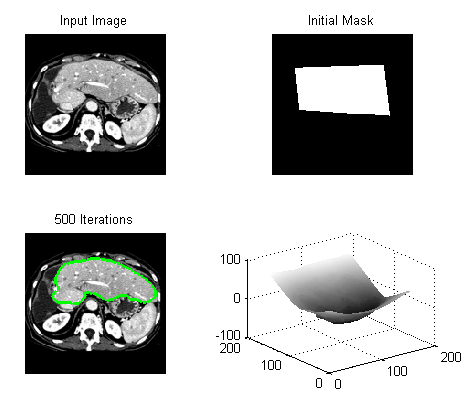
\includegraphics[scale=0.6]{images/matlab.png}
	\caption{MATLAB user interface showing four subfigures with the input image, the initial mask, the current zero level set interface superimposed on the input image and the current level set surface in 3D}
	\label{fig:matlab}
\end{figure}

The level set function $\phi$ is then initialised to a signed distance function of this mask, and iteration of the level set equation begins for a fixed number of iterations (also user-definable). Reinitialisation of the level set is performed once every 50 iterations, and the current level set contour and surface are displayed every 20 iterations.

The derivatives are calculated by subtracting shifted matrices of $\phi$ from $\phi$ (or vice-versa). Note how derivatives are not calculated in an element by element fashion.

Finally, the user has the option of downsampling the input image in order to speed up the computation.



	\subsection{C}
Initially C code was written 


\section{Parallel Implemention}
	\subsection{Block and Grid Sizes}
	\subsection{Shared Memory}